% Straight up stealing preamble from Eli Holmes 
%%%%%%%%%%%%%%%%%%%%%%%%%%%%%%%%%%%%%%START PREAMBLE THAT IS THE SAME FOR ALL EXAMPLES
\documentclass{article}

%Required: You must have these
\usepackage{Sweave}
\usepackage{graphicx}
\usepackage{tabularx}
\usepackage{hyperref}
\usepackage{natbib}
%\usepackage[backend=bibtex]{biblatex}
%Strongly recommended
  %put your figures in one place
 
%you'll want these for pretty captioning
\usepackage[small]{caption}

\setkeys{Gin}{width=0.8\textwidth}  %make the figs 50 perc textwidth
\setlength{\captionmargin}{30pt}
\setlength{\abovecaptionskip}{0pt}
\setlength{\belowcaptionskip}{10pt}
% manual for caption  http://www.dd.chalmers.se/latex/Docs/PDF/caption.pdf

%Optional: I like to muck with my margins and spacing in ways that LaTeX frowns on
%Here's how to do that
 \topmargin -1.5cm        
 \oddsidemargin -0.04cm   
 \evensidemargin -0.04cm  % same as oddsidemargin but for left-hand pages
 \textwidth 16.59cm
 \textheight 21.94cm 
 %\pagestyle{empty}       % Uncomment if don't want page numbers
 \parskip 7.2pt           % sets spacing between paragraphs
 %\renewcommand{\baselinestretch}{1.5} 	% Uncomment for 1.5 spacing between lines
\parindent 0pt% sets leading space for paragraphs
\usepackage{setspace}
%\doublespacing

%Optional: I like fancy headers
\usepackage{fancyhdr}
\pagestyle{fancy}
\fancyhead[LO]{How do climate change experiments actually change climate}
\fancyhead[RO]{2016}
 
%%%%%%%%%%%%%%%%%%%%%%%%%%%%%%%%%%%%%%END PREAMBLE THAT IS THE SAME FOR ALL EXAMPLES

%Start of the document
\begin{document}

% \SweaveOpts{concordance=TRUE}
 \bibliographystyle{/Users/aileneettinger/citations/Bibtex/styles/nature.bst}
\title{How do climate change experiments actually change climate?} % Paper 1/Large group paper from Reconciling Experimental and Observational Approaches for Climate Change Impacts

\author{A. K. Ettinger,I. Chuine, B. Cook, J. Dukes, A. Ellison, M. Johnston, A.M. Panetta,\\ C. Rollinson, Y. Vitasse, E. Wolkovich}
%\date{\today}
\maketitle  %put the fancy title on
%\tableofcontents      %add a table of contents
%\clearpage
%%%%%%%%%%%%%%%%%%%%%%%%%%%%%%%%%%%%%%%%%%%%%%%%%%%

\section* {Aim}

The aim is to write a Concept/Synthesis Paper, for Nature Climate Change, about maximizing benefits of field-based climate change experiments. We argue that there is a need to improve our understanding of how climate is actually altered by these experiments, particularly if we wish to use these experiments to forecast biological impacts of climate change. %yann: perhaps also to determine which methods of warming alter the least other climatic variables or to define the most appropriate method regarding the focus of the study (phenology, growth, survival etc)?%annmarie: Somewhere in this paper,  we should discuss that is important that “how” climate variables are modified relative to the predicted change under various emission scenarios is important.  Thus, the “how” should be not only the direction and magnitude of the variable change but also the extent to which the change mirrors change projected for the region in which the experiment took place). build up a discussion of studies that report only mean shifts in temperature in the intro. 

%EMW: Overall, looking great! I think we just now need to work on fine-tuning pieces, slimming long sentences and adding a little pep into here and there. 

\section* {Introduction}
% EMW: Some changes below -- tried to break up the two long, complicated sentences. I think we also need a little more intro to climate change here and acknowledgment that it IS already changing. Adjust so it reads more like: climate change is shifting things, future change will be even bigger with cascading effects...
\par Future climate change is expected to cause dramatic alterations to Earth's biota. The physiology, distribution, and abundance of organisms will shift, and likely cause cascading community and ecosystem effects \citep{thomas2004,parmesan2006,sheldon2011,urban2012}. Much uncertainty remains, however, about how particular individuals, populations, communities, and ecosystems will respond. These uncertainties make predicting ecological responses to the climate change one of the most significant challenges facing biology today.
% EMW: See quick (could be much better) changes below to better handle temperature and precipitation in this paragraph. Much work is on temperature because that's a known, relatively easy to predict effect, at least when compared to precipitation (we may or may not want to sneak this in). 

\par One major way to understand and forecast future biological conditions is through in situ experimental climate manipulations. Most of these studies have focused on manipulations to replicate higher temperatures. Commonly used field techniques for this include passive warming, such as open-top chambers, and active warming methods, including forced air, soil cables, and infra-red radiation. Passive warming methods have the benefits of being easy to deploy and relatively inexpensive, making it possible to set them up in more remote and challenging-to-access areas. In contrast, active warming methods require extensive infrastructure and are generally costly, yet they have been shown to be the most controlled, consistent, and ``true to climate change predictions" \citep{kimball2005,kimball2008,aronson2009,wolkovich2012}. Recently, interest has also expanded to understand changing precipitation. Today, many active warming methods are frequently combined with precipitation manipulations, including drought, snow-removal, and supplemental precipitation treatments, in an effort to create climatic conditions such as those forecasted under future climate change scenarios \citep{price1998,cleland2006,sherry2007,rollinson2012}.

% EMW: I am not sure about mixing the pros and cons here .... it makes the transition to the next paragraph really hard and I am not sure of the point of the paragraph then, or where it should come. I did what I could -- see what you think.
\par Experimental in situ climate warming manipulations offer several advantages over other approaches---such as long-term observational data and growth chamber studies---for understanding biological impacts of climate change. In particular field experiments replicate the natural environment while allowing effects of temperature and precipitation to be isolated from other environmental changes. In addition, a range of warming and/or precipitation treatments can be applied, such that potential non-linear relationships of climate responses can be evaluated. These advantages come at a cost, however. The most accurate experimental in situ climate manipulations (i.e., active warming methods) are logistically challenging and expensive \citep{aronson2009}. Even with extensive resources it is often difficult to design, implement, and monitor replicated experiments that consistently apply the intended climate manipulations. Yet, despite these limitations, field warming experiments offer some of our best estimates of future biological responses to warming. 

\par Given warming experiments' high value in estimating ecological responses scientists and others often wish to extrapolate the results of in situ climate change experiments to forecast how organisms and ecosystems will respond to particular climate change scenarios. Even in cases where this is not the explicit goal of warming and other climate change experiments, it would be incredibly useful to be able to apply knowledge gained from these experiments to improve our understanding and forecasting of how anthropogenic warming will affect species' performance (growth, survival) and distributions. Our ability to make this application, however, is currently limited. This is because we lack a detailed assessment of exactly how experimental warming treatments alter climate and the extent to which these manipulations accurately model the real world, both present and future. 

\par To realize the forecasting potential of climate change experiments, a more nuanced understanding of how climate change experiments actually change climate is critical. Towards this goal we carried out a full literature review to identify all active field warming experiments then obtained daily (or sub-daily) climate data from as many as possible (we obtained data for 12/XX total identified experiments, see Supplemental Materials for details). We are thus able to show, for the first time, the complex ways that climate is altered by active warming treatments, both directly and indirectly. The data we use are from experiments in North America and Europe that were collected between 1991 and 2014, and have been merged into a new, publicly available database (names GOOBER). We then discuss the challenges of interpreting biological implications of experimental shifts in climate, when these climate manipulations are more complex then simple shifts in the mean. Finally, we make recommendations for future climate change experiments.
% Need to give the database a name!

\section* {Complications in extrapolating experimental climate change}
Climate change experiments often include detailed monitoring of climate variables at the plot level, yielding large amounts of data, such as daily or hourly temperature and other climate variables, over the course of the experiment. However, biologists are generally interested primarily in the biological responses associated with each treatment (e.g. growth, abundance, or phenology of a species). Not surprisingly, then, authors typically provide detailed information on the observed biological responses, and report only the mean change in climate over the course of the experiment and whether or not that mean change matched their target level of change \citep{price1998,clark2014a,clark2014b,rollinson2012}. 

\par Though the published focus is often on shifts in the mean, the imposed climate manipulations result in much more complex shifts of climate. The magnitude of change experienced by organisms in these manipulations is likely to vary in time and space, and the equipment required to conduct these manipulations can also alter climate at the plot level. % EMW: Last sentence is a lot here -- can you break into two? One would be on changes to climate and the other can make the leap to organisms.

\subsection* {Treatments vary over time}
The common practice of reporting only the mean temperature difference, across the duration of the study, may hide variations in annual, seasonal, and daily minimum and maximum temperatures.There are frequently strong seasonal variations in experimental warming effects (Figure 1). This can occur because treatments are not applied consistently over the year, either because heat applications are frequently shut off during some seasons such as when snow cover is present \citep[e.g.][]{clark2014a,clark2014b} (Yann and Isabelle- could you recomend some studies from Europe that also use this methodology) or because some heating methods, even if left on throughout the year, are not capable of applying consistent warming year-round (e.g. infrared radiation, CITATION- Christy, Yann, and/or Jeff could you suggest 1 or 2?). Furthermore, seasonal precipitation patterns can alter the effectiveness of warming treatments (CITATION- Christy, Yann, and/or Jeff could you suggest 1 or 2?). % it is likely that this would yield different effects than if heating were turned on during winter (because then you change soil nutrient mineralization which might be important in winter and so change nutrient availability and moisture for the growing season ).
% EMW: Can you show any of the diurnal changes you mention? At least in the supp?

\par In addition to seasonal patterns, experimental warming effects can vary widely across longer timescales, such as among years (Figure 2). This is probably due to interactive effects of warming treatments and other aspects of weather that may vary annually. For example, Hoepner and Dukes (2012) found that infrared heaters failed to achieve the target temperatures during rainstorms. 

\par Warming treatments can also vary on shorter timescales, such as within a day. This often leads to a decrease in the diurnal temperature range within experimental plots, compared with ambient conditions \citep{hoeppner2012}. This may be similar to what is projected for parts of world \citep{ipcc2013}. However, this will likely vary spatially, as some regions have experienced higher daytime warming than nighttime warming, whereas others have experienced the opposite\citep{ipcc2013}. 

\par A detailed comparison of projections versus observations in climate change experiments is lacking. Thus, it is unknown how divergent these annual, seasonal, and daily variations may be from real (i.e. non-experimental) climate patterns.  %there are several recent papers showing the importance of diurnal over nocturnal temperature on phenology. %EMW: Adjust above paragraph to focus also what we need to do. 

\par Anne Marie- please write a paragraph on your suggested discussion "that 3-5 year studies may not capture ultimate, long-term responses that may actually be in the opposite direction to short-term responses.  Cite recent Global Change Biology paper by Harte et al.  Ideally, we want to run studies long enough to capture population-level responses to warming." I would love to work this in and I think you are the one to write it!

\subsection* {Treatments vary in space}
In addition to temporal variation, there can be spatial variation in experimental warming effects, such that extrapolation of experimental warming to forecast climate change impacts may not be a straightforward space-for-time substitution. For example, our database contains three studies that used a blocked designs, allowing us to examine spatial variation in the amount of warming (i.e. the difference between treatment and control plots within a block). We found that the amount of warming may vary by more than one degree among blocks (Figure 2, Table 1), resulting in lower warming treatments that varied almost 100\% of their target temperature and higher warming treatments varying 20\% (EMW: I am eye-balling, give exact values).% EMW: I offered one way to build on the finding, you could come up with many others instead -- I think it is important to just point it out a little more. 

\par Presumably, there will be spatial variation in future climate change effects, given that warming to date has varied spatially \citep{ipcc2013}).  Accurate extrapolation of climate change experiments may therefore depend on the extent to which experiments encompass a representative amount of existing natural variation (e.g. gradients in slope, aspect, etc) present at the scale at which the extrapolation is being made. 

\par An added complication is that inferences made from space-for-time substitutions are frequently invalidated, when they have been tested with empirical evidence \citep{johnson2008}. When experimental manipulations aimed at understanding future responses are imposed in a spatially varying environment, we need to be explicit about what assumptions are made in this modified space-for-time substitution, think critically about whether these assumptions are realistic, and then carefully interpret results in light of these assumptions. (Aaron- do you think we need more here about space-for-time substitution and its problems? If so, what? or do you have citations we should add?). There is also documented small-scale variation in the amount of warming, within experimental plots, at least from passive warming studies \citep {marion1997}.

\subsection* {Experimental infrastructure alters climate}
The experimental structures themselves alter temperature and other important biotic and abiotic variables, in ways that are not generally examined or reported in experimental warming studies. The possible existence of these effects are widely acknowledged, and some studies include `shams' or `disturbance controls' to account for them. However, the magnitude of structural effects on climate are rarely discussed or interpreted in climate change studies.

\par To investigate the magnitude of these effects, we compared temperature and soil moisture data from four active warming studies at two sites: Duke Forest and Harvard Forest\citep{farnsworth1995,clark2014a, marchin2015, pelini2011}. These four were the only studies in our database that included two types of control plots: structural controls (i.e. `shams' or `disturbance controls,' which contained all the warming infrastructure, such as soil cables or infrared heating units but with no heat applied) and ambient controls with no infrastructure added (see Supplemental Materials for details).  

\par We found that experimental structures altered air and soil temperatures in opposing ways:  air temperatures were higher in the structural controls, compared with the ambient air with no structures installed, whereas soil temperatures were lower in the structural controls compared with ambient soil (Figure 3). This was consistent across the different temperature models we fit (mean, minimum, and maximum), and the sign of the effects was consistent across study-sites and months, although the magnitude varied among sites (Table 3) and across seasons (Figure 3). Soil moisture was lower in structural controls compared with ambient conditions (Figure 1S). 

\par In addition to these documented effects, experimental structures may alter conditions by creating shade, intercepting precipitation, and altering herbivory and other biotic interactions. Further documentation and analysis of the effects of these experimental structures on abiotic and biotic factors, as well as in depth interpretation of how these effects may alter focal variables, is an important next step for climate change experimentation, particularly if we wish to apply results to forecasting.

\section* {Secondary effects of climate change manipulations}
Climate change experiments often manipulate one or two climate variables, such as temperature and precipitation. However, as scientists who have conducted these experiments have likely experienced, climatic variables are nearly impossible to completely isolate from one another.  Temperature, for example, interacts with precipitation to alter the abiotic environment; Rollinson et al (2012) observed that a twenty percent increase in precipitation reduced mean hourly temperatures by 0.3 degrees Celsius over the course of their two-year experiment. 
% EMW: Need to move this below sentence or make transition into it better ...
Ideally, experimentally induced changes in other variables would be realistic; for example, the experimental treatment should not decrease moisture in an area projected to get wetter. At the very least, it is important to quantify the secondary effects of applied manipulations.  

\par Precipitation treatments typically reduce temperatures in climate change manipulations, as described above \citep[e.g.][]{sherry2007,rollinson2012}, but the magnitude of this effect can vary in space and time (Figure 2S). Experimental warming  reduces vapor pressure deficit and soil water content \citep[e.g. Figure 3S][]{sherry2007,morin2010,templer2016}. Miriam: please try adding a discussion of your soil moisture analysis here! The magnitude of these effects are also likely to vary in space and time. %EMW: Can you add a discussion of the modeling consequences here? Scientists have non-orthogonal treatments! They may need more than an RM-ANOVA to fully understand their results .... 

\par Warming and precipitation treatments can also alter plant community composition, which can produce additional secondary effects that alter climate. For example, tree composition shifted after three years of warming and modified precipitation treatments \citep{rollinson2012}. These shifts in composition may change competitive dynamics and, in turn, affect resource levels, such as moisture in the soil.  It can be difficult to tease out limiting resources and abiotic and biotic drivers of biological responses, but understanding the effects of an experimental treatment on these interrelated variables is critical when trying to determine mechanistic explanations for observed responses to warming. %EMW: AnneMarie I think has sad that shrubs can also shade soil, producing cooler soils.

\section* {Biological implications}
\par We have highlighted a suite of factors that complicate interpretations of warming experiments. We argue that these largely unintended alterations are important for scientists to fully understand and report in their research (Figure 4). This is especially important because unintended climate alterations are likely to have biological implications, including for many of the major responses studied in warming experiments.

\par Shifted plant phenology is often reported in warming experiments. Yet understanding exactly what drives shifted phenology may be more complicated than simply comparing shifts to the direct warming effects of the experiment. This is because phenology is likely to be altered in opposing ways by the increased air temperatures---which generally advance phenology---and decreased soil moisture---which may delay phenology---characterized by warming treatments. Indeed, these opposing drivers may be responsible for the observed discrepancy between observational and experimental phenology responses to warming\citep{wolkovich2012}. In addition, plant phenology responds to minimum temperatures, as well as mean and maximuma, and this may also play a role in the discrepency between observational and experimental studies \citep{shen2016,matthews2016}. Lizzie, Aaron, Yann, Isabelle-Please recommend other citations for this! %EMW: Check Sherry or Craine for citations on soil moisture impacts on phenology. Lots of cites that warming advance phenology!

\par Plant growth is also likely to be altered in opposing ways by the increased air temperatures and decreased soil moisture levels in experimentally warmed plots. For example, with warming and decreased VPD, stomata closure may reduce sapflow and growth \citep{templer2016}. Even small shifts in temperature may have a big effect, since the photosynthetic response to temperature is nonlinear \citep{berry1980}. %EMW: Nice paragraph!

\par Direct and indirect effects of climate change experiments are also likely to affect soil respiration in ways that may alter net mineralization and therefore have other cascading effects. Yann: please add a few sentences and citations here!

\par Other biotic interactions are also likely to be affected by direct and indirect affects of climate change treatments. For example, Hoeppner and Dukes  (2012) found that rodent disturbance varied by warming treatment (as well as year) in their climate change experiment. Aaron, Anne-Marie, Yann, and/or Jeff- please add other examples (with citations) if you can think of some good ones? A critical question is the extent to which these shifts in biotic interactions (and their effects on focal responses) are accurate forecasts of future shifts that are likely to occur with climate change, or due to side-effects that are unlikely to occur outside of experimental systems.

\section* {Recommendations for future climate change experiments}
 \par Climate change experiments provide invaluable information about biological responses to climate change, yet our results highlight that we do not fully explore the ways in which these climate change experiments are actually altering climate. These complications should not suggest that experimental climate change studies are not worthwhile. Instead we believe these complications and the relating climate data provide the foundation to designing better experiments, and gaining the most knowledge and utility from existing experiments. Below we describe recommendations to improve implementation, interpretation, and communication of future climate change experiments.
 
\par\textit{Design realistic manipulations} by consulting climate change projections for the study region, and selecting warming and precipitation treatment methods that most accurately mimic anticipated changes. When it is not possible to match anticipated changes in climate, studies should report how imposed treatments compared to projected changes. In addition, the timing of these treatments should be carefully considered and ideally should match forecasts. If it is not possible to apply continuous treatments throughout the study, the seasonality and timing of treatments should be explicitly reported. We found that only 4/12 studies used shams, yet all of them showed effects of shams. %EMW: Add more here -- thus, everyone should do them, even if they are a pain. Better to have accurate results on fewer treatments than inaccurate results on more treatments or plots etc.!!

\par\textit{Include both structural and ambient controls} and collect, use, and report data collected within them. This will facilitate separating mechanisms due to experimental design from mechanisms due to actual shifts in climate.  
\par\textit{Maximize the length of climate change experiments} by running them for as long as possible. This will allow study of how inter-annual variations interact with climate change treatments, especially when looking at non-linear and multiyear processes such as phenology. It will also allow us to understand how long-term responses may differ from  transient ones. Citations, anyone?
\par\textit{Collect fine-scale climate data}, at least twice daily, and ideally hourly, to allow for minimum and maximum values to be analyzed and interpreted, in addition to mean values.
 \par\textit{Publish high quality, usable data and metadata} such that data can easily be shared and used by others. In the metadata, report the number and cause of missing data points for climate, especially those collected in warming treatments. (For example, are data missing because the heaters went out, or because rodents at the sensors?) Report the timing of applied warming treatments (i.e. exact start and end dates, within and across years), as well as variations in daytime and nighttime and seasonal variations in climate variables. 
\par\textit{Consider implementing and following community standards for reporting climate data} Do we have community standards for climate data? Ben- do you have any ideas of resources for this?
When studying biological implications of a global challenge as large as climate change, it facilitate progress if we can design, run, and report experiments in such a way that we can eventually create global dataset. This recommendation stems from our work gathering and analyzing data from many climate change experiments. We found that studies report a diverse range of climate variables, collected in different ways (i.e. soil temperature collected at different depths; soil moisture using different units and methods). It has been difficult to synthesize these data in a comprehensive way that can fully address important questions. 

\par Documenting biological impacts of climate change has over a 20 year history in ecology today. Over this time situ field experiments have been critical in making the mechanistic link between warming and a number of major biological impacts---changes in productivity, soil respiration, the phenology of plant and animals and shifted community and ecosystem dynamics. Yet as climate change across the globe continues with projected warming of XX C over the next 80 years, ecologists are challenged to not only document impacts but make quantitative robust predictions. Our ability to meet this challenge requires building on the data from current and past experiments to best understand how altered climate changes ecological processes and build better experiments. As a first step, we have compiled the first database of fine-scale climate data from warming experiments and shown how time, space and artifacts may hinder simple interpretations of climate change experiments. The next steps require the ecological community to build on these data and their findings to develop and use new approaches in the experiments to provide more accurate estimates of altered climate in theses experiments and in turn, more accurate estimates of critical biological changes. 

\bibliography{/Users/aileneettinger/citations/Bibtex/mylibrary}
\clearpage
\section* {Tables}

% EMW all tables should go into supp and give the results parenthetically in main text (sweavedemo has an example of how to do this). Also be SURE TO GIVE ERROR DF throughout. 

% latex table generated in R 3.2.4 by xtable 1.8-2 package
% Thu Sep 29 18:32:48 2016
\begin{table}[ht]
\centering
\begin{tabular}{lrrr}
  \hline
 & Chisq & Df & Pr($>$Chisq) \\ 
  \hline
(Intercept) & 861.834 & 1.000 & 0.000 \\ 
  temptreat & 431.799 & 3.000 & 0.000 \\ 
  block & 5.795 & 2.000 & 0.055 \\ 
  temptreat:block & 43.094 & 6.000 & 0.000 \\ 
   \hline
\end{tabular}
\caption{Effects of warming vary by block, as summarized by a linear mixed effects model of mean soil temperatures, with year and site as nested random effects} 
\end{table}
% latex table generated in R 3.2.4 by xtable 1.8-2 package
% Thu Sep 29 18:32:48 2016
\begin{table}[ht]
\centering
\begin{tabular}{lrrr}
  \hline
 & Chisq & Df & Pr($>$Chisq) \\ 
  \hline
(Intercept) & 1455.294 & 1.000 & 0.000 \\ 
  temptreat & 126.093 & 3.000 & 0.000 \\ 
  year & 16.676 & 1.000 & 0.000 \\ 
  temptreat:year & 61.646 & 3.000 & 0.000 \\ 
   \hline
\end{tabular}
\caption{Effects of warming vary by year, as summarized by a linear mixed effects model of mean soil temperatures, with year and site as nested random effect} 
\end{table}\par The below are all tables related to the sham and ambient comparisons. i want to include more information in the tables, probably (random effects- intercepts, and variance), and most will be in the supplemental (perhaps just the mean soil and air in the main text?)
.
\par 
% latex table generated in R 3.2.4 by xtable 1.8-2 package
% Thu Sep 29 18:32:52 2016
\begin{table}[ht]
\centering
\begin{tabular}{rrrr}
  \hline
 & Estimate & Std. Error & t value \\ 
  \hline
(Intercept) & 12.674 & 1.632 & 7.766 \\ 
  controltypeambient & -0.356 & 0.092 & -3.859 \\ 
   \hline
\end{tabular}
\caption{Summary of linear mixed effects model testing difference in mean air temperatures of structural controls compared with ambient controls (i.e.with no control chambers or warming infrastructure in place). The model included a fixed effect of control type and an intercept-only random effect of studysite to account for study and measurement, as well as environmental, differences.} 
\end{table}
\par
% latex table generated in R 3.2.4 by xtable 1.8-2 package
% Thu Sep 29 18:32:52 2016
\begin{table}[ht]
\centering
\begin{tabular}{rrrr}
  \hline
 & Estimate & Std. Error & t value \\ 
  \hline
(Intercept) & 11.312 & 1.366 & 8.283 \\ 
  controltypeambient & 0.425 & 0.068 & 6.285 \\ 
   \hline
\end{tabular}
\caption{Summary of linear mixed effects model testing difference in mean soil temperature (at the shallowest depth measured) of structural controls compared with ambient controls. The model included a fixed effect of control type and an intercept-only random effect of studysite to account for study and measurement, as well as environmental, differences.} 
\end{table}
\par
% latex table generated in R 3.2.4 by xtable 1.8-2 package
% Thu Sep 29 18:32:52 2016
\begin{table}[ht]
\centering
\begin{tabular}{rrrr}
  \hline
 & Estimate & Std. Error & t value \\ 
  \hline
(Intercept) & 7.161 & 1.381 & 5.186 \\ 
  controltypeambient & -0.389 & 0.092 & -4.236 \\ 
   \hline
\end{tabular}
\caption{Summary of linear mixed effects model testing difference in minimum air temperatures of structural controls compared with ambient controls (i.e.with no control chambers or warming infrastructure in place). The model included a fixed effect of control type and an intercept-only random effect of studysite to account for study and measurement, as well as environmental, differences.} 
\end{table}\par
% latex table generated in R 3.2.4 by xtable 1.8-2 package
% Thu Sep 29 18:32:52 2016
\begin{table}[ht]
\centering
\begin{tabular}{rrrr}
  \hline
 & Estimate & Std. Error & t value \\ 
  \hline
(Intercept) & 10.493 & 1.334 & 7.866 \\ 
  controltypeambient & 0.346 & 0.068 & 5.089 \\ 
   \hline
\end{tabular}
\caption{Summary of linear mixed effects model testing difference in minimum soil temperature (at the shallowest depth measured) of structural controls compared with ambient controls. The model included a fixed effect of control type and an intercept-only random effect of studysite to account for study and measurement, as well as environmental, differences.} 
\end{table} 
% latex table generated in R 3.2.4 by xtable 1.8-2 package
% Thu Sep 29 18:32:52 2016
\begin{table}[ht]
\centering
\begin{tabular}{rrrr}
  \hline
 & Estimate & Std. Error & t value \\ 
  \hline
(Intercept) & 18.187 & 1.899 & 9.576 \\ 
  controltypeambient & -0.322 & 0.098 & -3.290 \\ 
   \hline
\end{tabular}
\caption{Summary of linear mixed effects model testing difference in maximum air temperatures of structural controls compared with ambient controls (i.e.with no control chambers or warming infrastructure in place). The model included a fixed effect of control type and an intercept-only random effect of studysite to account for study and measurement, as well as environmental, differences.} 
\end{table}
% latex table generated in R 3.2.4 by xtable 1.8-2 package
% Thu Sep 29 18:32:52 2016
\begin{table}[ht]
\centering
\begin{tabular}{rrrr}
  \hline
 & Estimate & Std. Error & t value \\ 
  \hline
(Intercept) & 13.599 & 1.670 & 8.145 \\ 
  controltypeambient & 0.572 & 0.076 & 7.532 \\ 
   \hline
\end{tabular}
\caption{Summary of linear mixed effects model testing difference in maximum soil temperature (at the shallowest depth measured) of structural controls compared with ambient controls. The model included a fixed effect of control type and an intercept-only random effect of studysite to account for study and measurement, as well as environmental, differences.} 
\end{table}

\clearpage
\section* {Figures}

 \begin{figure}[p]
     \centering
 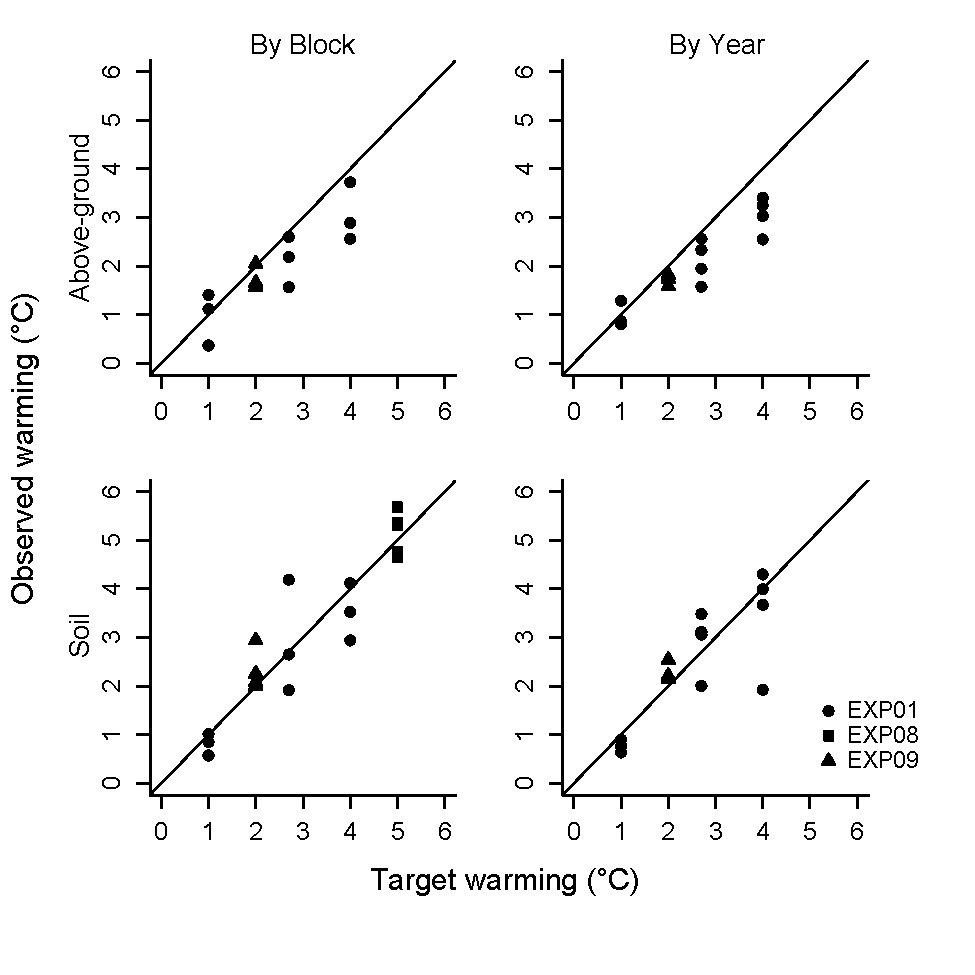
\includegraphics{../figures/BothWarmingbyblockyear.pdf}    
 \caption{The amount of warming (i.e. the difference between treatment and control plots, within each block) varies among blocks (left panels), as well as among years (right panels). See Tables 1 and 2 for statistical differences.} %EMW: line is 1:1? Also, we should have a map of the sites somewhere? New Figure 1?
 \end{figure}
\clearpage
 \begin{figure}[h]
     \centering
 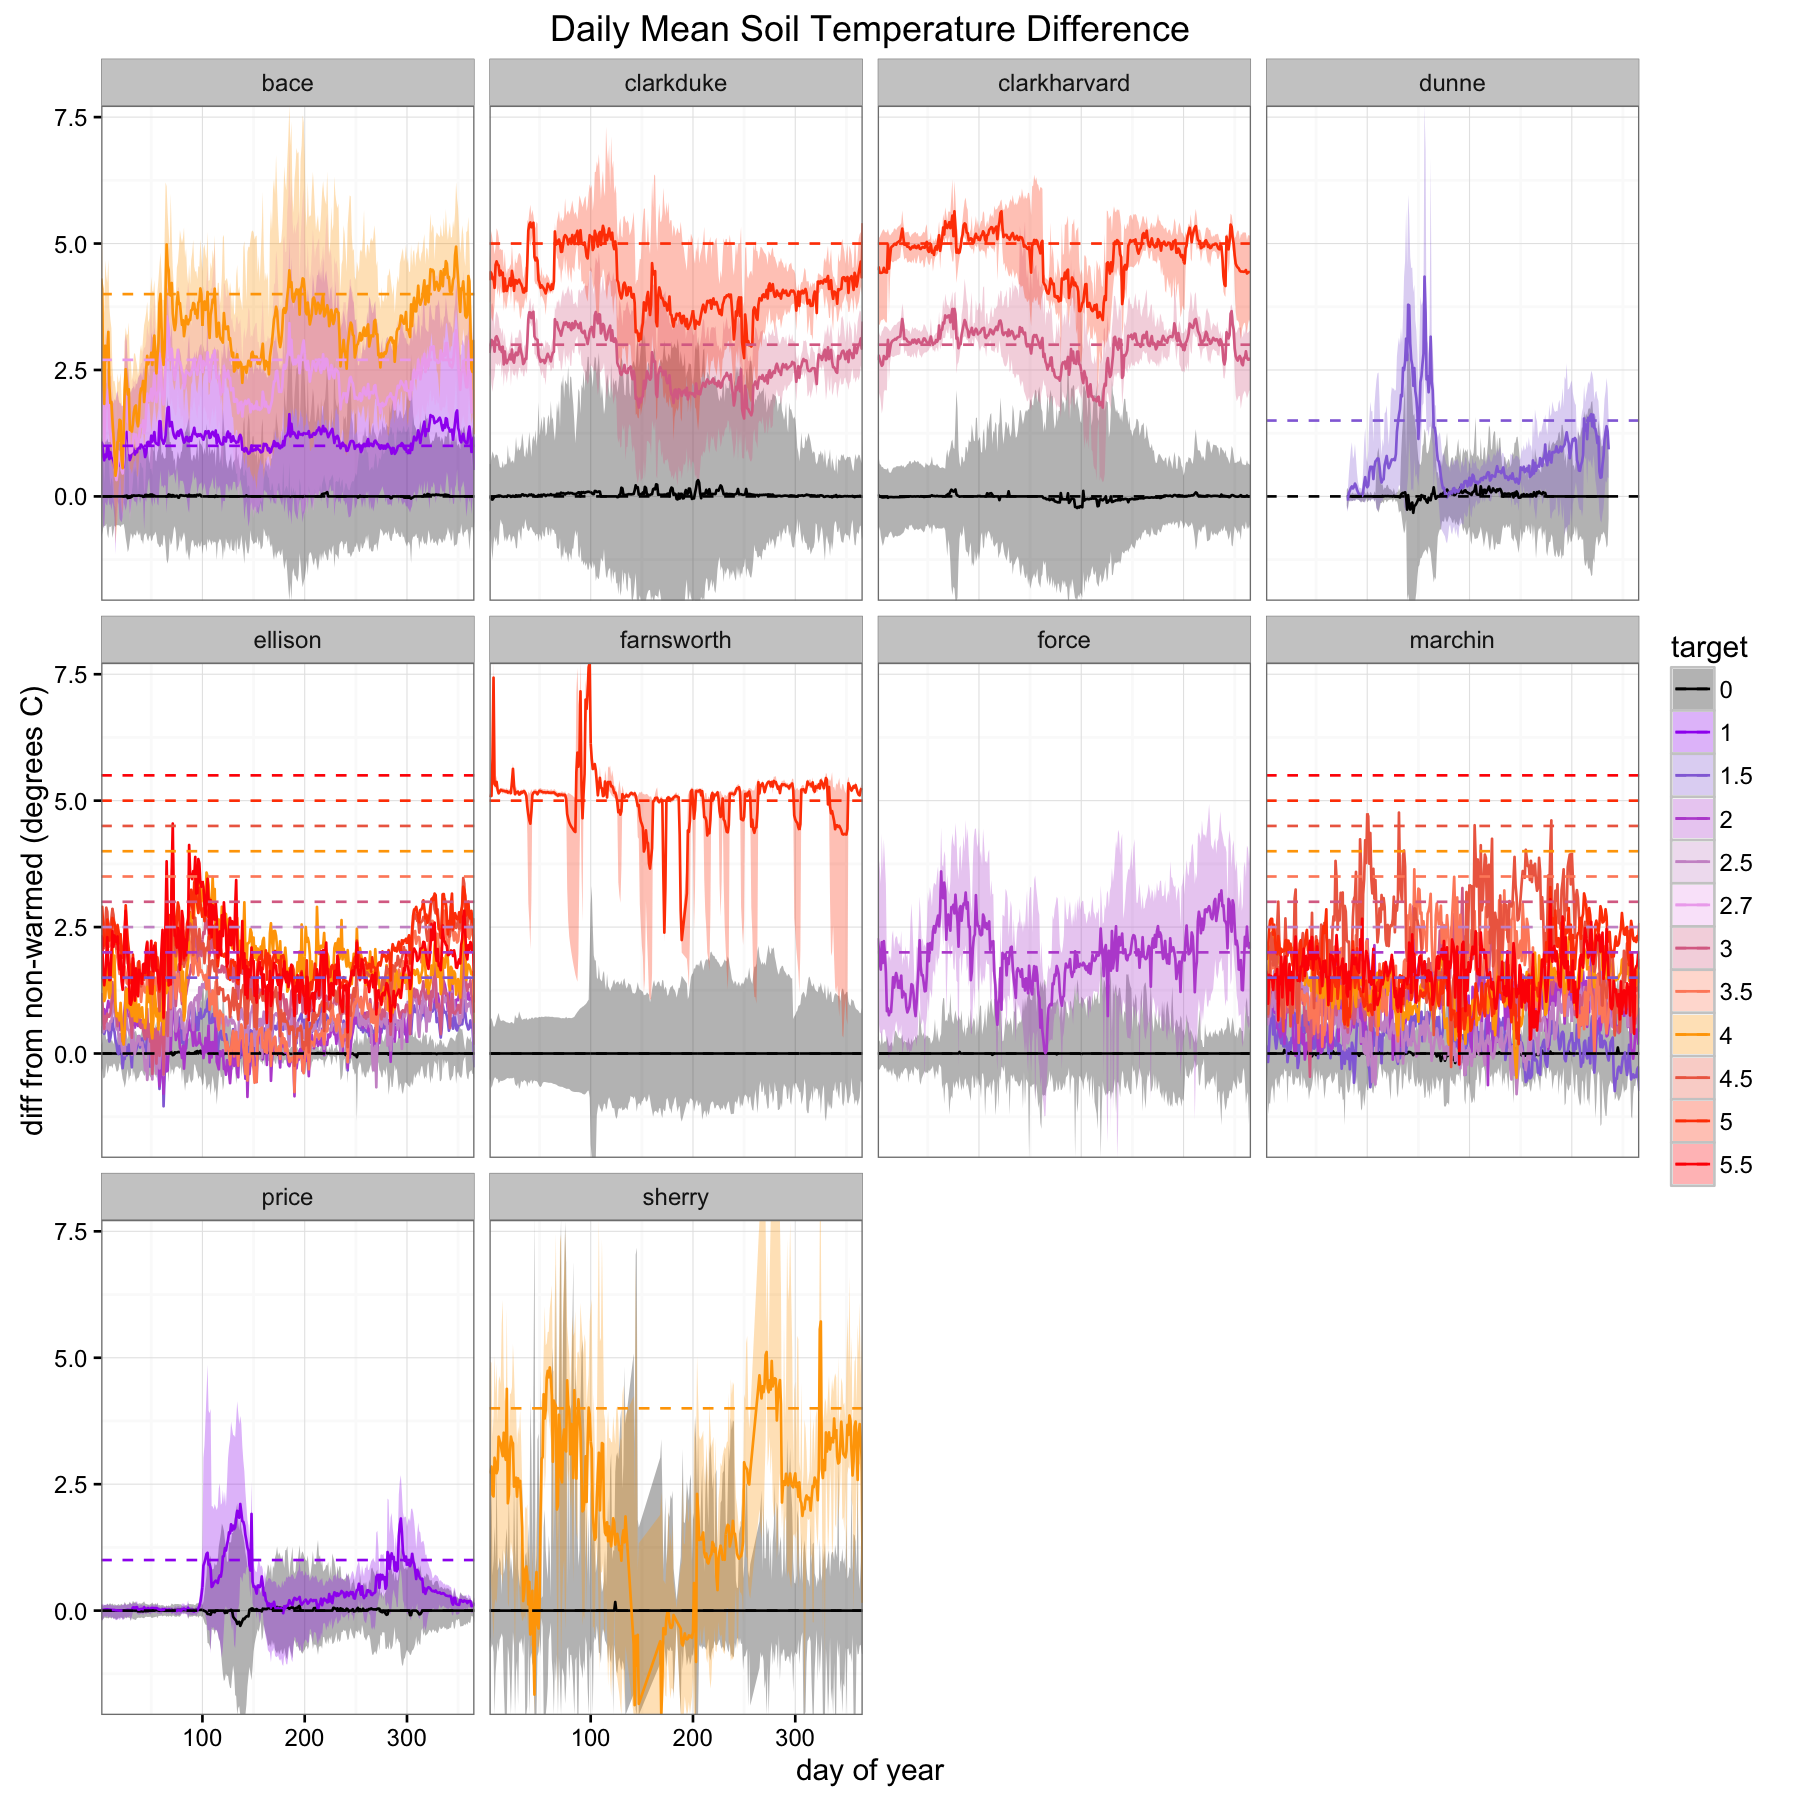
\includegraphics{../figures/Exploratory_TimeSeries_SoilTemp1Mean_Deviation.png}    
 \caption{Time series of deviations from mean soil temperature over one year, in control (black line) and warming treatments with various target warming levels at 10 study sites.} %EMW: This figure is great -- you should make it sound more exciting when you mention it in the main text.
 \end{figure}
\clearpage
 \begin{figure}[h]
     \centering
 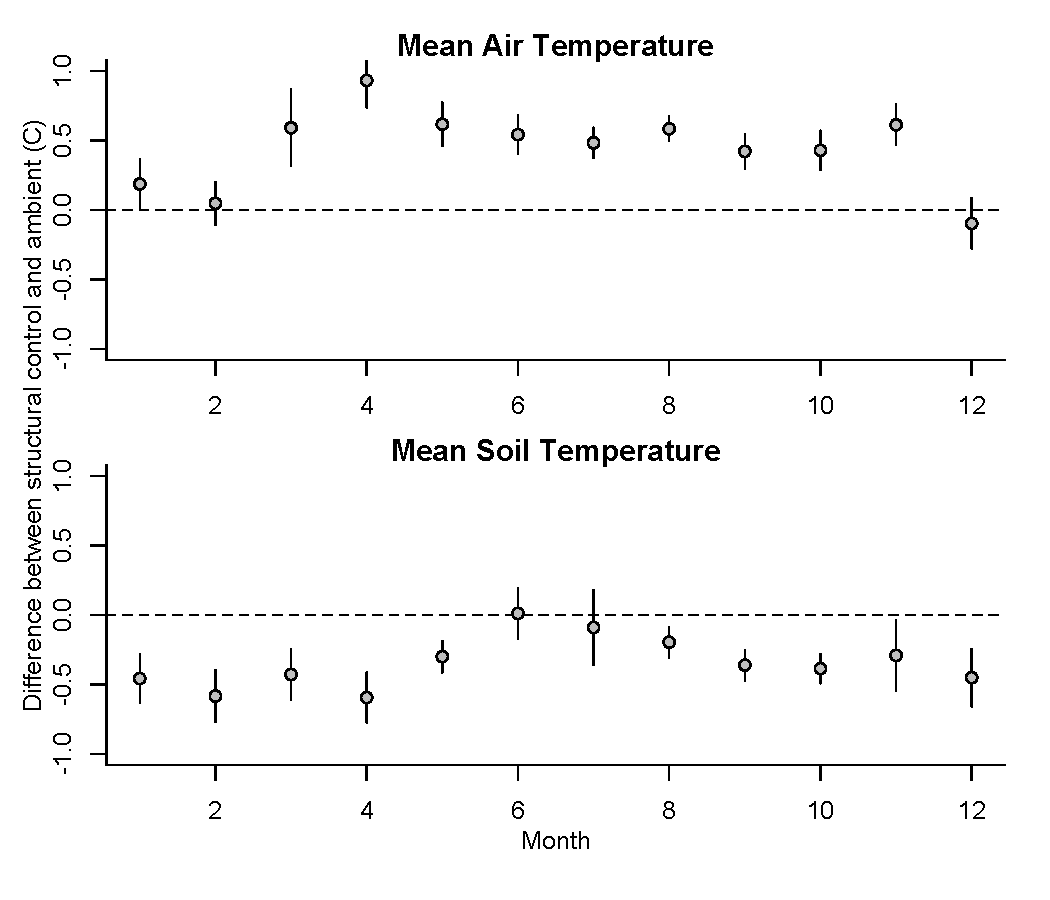
\includegraphics{../figures/ShamVSAmbient_mean.pdf}    
 \caption{Difference between mean air and soil temperatures in structural controls compared with ambient controls, with no control chambers or warming infrastructure in place. Air temperatures were higher, whereas soil temperatures were lower in the structural controls compared with ambient conditions. We show fixed effects from a mixed effects model that accounts for differences in experimental design and other factors among sites by including site as an intercept-only random effect (see Supplemental Materials for details). } % Add ref to table in supp for stats.
 \end{figure}
 \clearpage
 \begin{figure}[h]
     \centering
 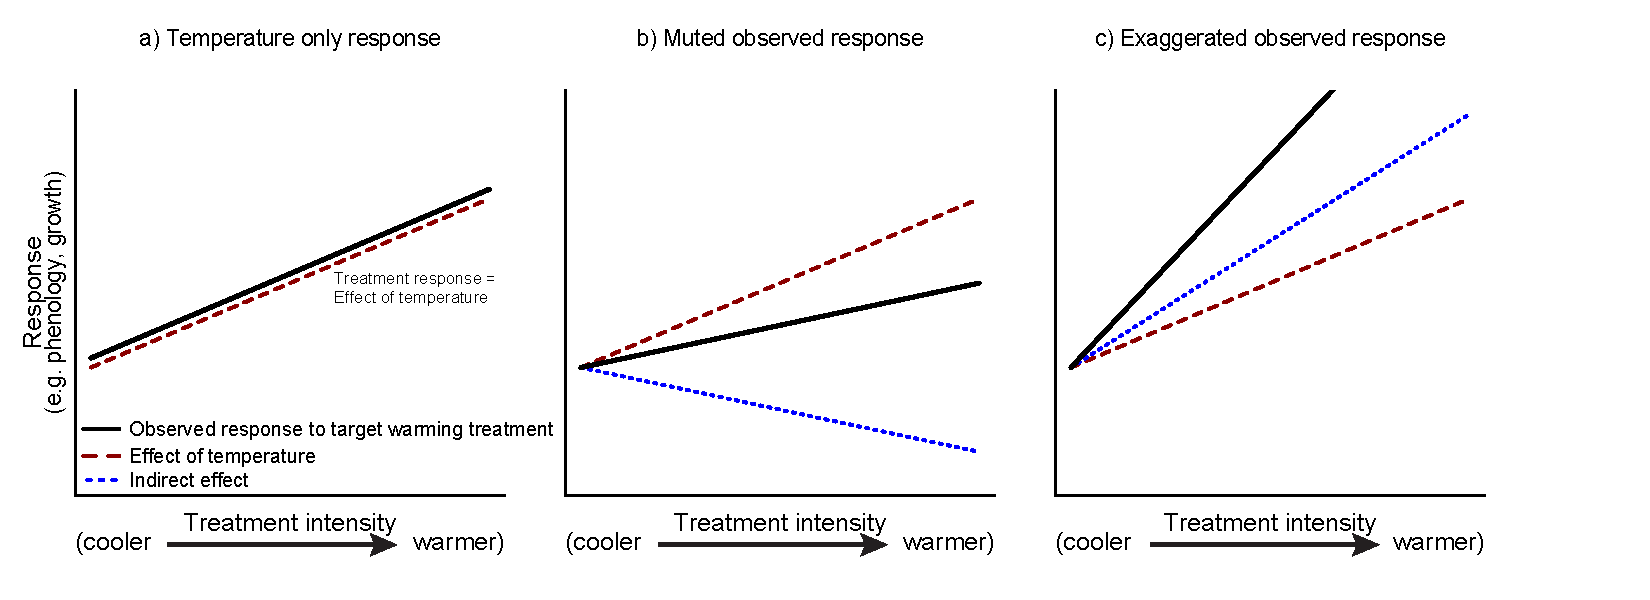
\includegraphics{../figures/DirIndWarmingEffects.pdf}    
 \caption{Experimental warming may cause biological responses to be muted or exaggerated, compared to direct responses to temperature alone, when indirect effects of experimental warming are also drivers of focal responses. For example, phenology may appear to be less sensitive to warming in experiments versus observational studies \citep{wolkovich2012} because experimental warming reduces soil moisture, perhaps more than natural warming.} 
 % EMW: Change the Y axis title so it's clearer -- effect of structural control (difference ....)? 
 % EMW: Explain phenology better (advances and delays) or just refer reader to main text for examples.
 \end{figure}
\clearpage
\section*{Supplemental Materials}
\subsection*{Description of database}
Search terms used and criteria for selecting the 12 studies that we ended up with. Climate variables included, and where database and metadata are housed.
\subsection*{Supplemental Methods}
\par\textit{Statistical methods}
\par Need description of block and year analyses (see Tables 1 and 2) 
To account for differences in the type of warming and other unmeasured site/study differences (e.g. forced air for Ellison and Marchin; heating cables for Farnsworth and ??), we fit linear mixed effects models with random effect of study-site. Response variables were daily soil or air temperature (models with daily  mean, minimum, and maximum were all fit) and , and the explanatory variable was control type (infrastructure or ambient). We used a random intercepts structure, so that the mean temperature was allowed to vary across study-sites. We fit models across the entire year, as well as separate models for each month to examine if effects varied seasonally.
%%%%%%%%%%%%%%%%%%%%%%%%%%%%%%%%%%%%%%%%
\end{document}
%%%%%%%%%%%%%%%%%%%%%%%%%%%%%%%%%%%%%%%%
